\documentclass{article}
\usepackage[utf8]{inputenc}
\usepackage{titlesec}
\usepackage{amsmath}
\usepackage{tikz}

%\setlength{\parindent}{0em}

\titleformat{\section}
{\normalfont\fontsize{12}{15}\bfseries}{\thesection}{1em}{}

\titleformat{\subsection}
  {\normalfont\fontsize{10}{15}}{\thesubsection}{1em}{}

\usepackage[style=ieee, sorting=ynt, doi=false,isbn=false,url=false,eprint=false, defernumbers=true]{biblatex}
\addbibresource{papers.bib}
\AtBeginBibliography{\small}

\title{Codec Classifier}
\date{November 17, 2023}

\begin{document}

\maketitle

This paper describes a classifier architecture consisting of an encoder and a decoder.  The word ``codec'' in the name Codec Classifier follows from merging the words en{\it co}der and {\it dec}oder.

\begin{figure}
  \begin{center}
  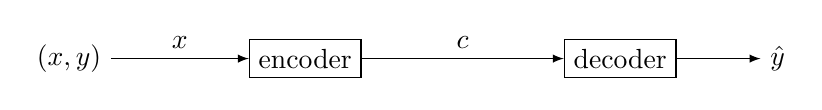
\begin{tikzpicture}[>=latex]
    \node at (-1,0) (x){$(x,y)$};
    \node at (2,0)[draw] (enc){encoder};
    \node at (6,0)[draw] (dec){decoder};
    \node at (8,0) (y){$\hat{y}$};
    \draw[->] (x.east) -- (enc.west) node[above,midway]{$x$};
    \draw[->] (enc.east) -- (dec.west) node[above,midway]{$c$};
    \draw[->] (dec.east) -- (y.west);
  \end{tikzpicture}
\end{center}
\label{fig:arch}
\caption{Structure of the codec classifier.}
\end{figure}

The architecture of the codec classifier is shown in Fig.~\ref{fig:arch}.  An input feature vector $x$ is input to the encoder, which outputs a codeword $c$, which is decoded to a predicted class label $\hat{y}$.  This classifier architecture is reminscent of a communication system.  In communication systems,
\begin{itemize}
  \item the codeword is a perfect representation of the message $x$,
  \item the channel corrupts the bits of the codeword, and
  \item the decoder attempts to recover the message $x$.
\end{itemize}
The decoder's ability to determine $x$ without errors depends on the extent of the channel distortion.

In the classification problem,
\begin{itemize}
\item the encoder may be lossy in the sense that $x$ may not be recoverable from $c$,
\item there is no channel, and
\item the decoder may also be lossy.
\end{itemize}
In classification, the goal is to identify the class $y$ associated with $x$.

In communication systems, mutual information is used as a metric to design schemes that make the best use of the channel.  For classification, we adopt the mutual information as a metric to design the encoder and decoder.  We also use the Bayes error.

Consider an encoder consisting of $d$ classification trees having binary codes in the leaves.  A tree with $r$ layers of decision nodes has $2^r$ leaf nodes.  The tree input $x$ selects a leaf node and the leaf's $r$-bit code is output.  Concatenating the results of $d$ trees together yields a $dr$-bit codeword $c$.   A tree with $r=1$ is called a stump.  A stump outputs one bit.  The parameters of a tree are the feature indexes $f_i$, thresholds $t_i$, and $r$-bit codes assigned to the leaves.  The tree output results from a sequence of decisions $x_{f_i} \leq t_i$.  When true, the decision tree is descended to the left child node and the right child node otherwise.  The classifier design problem chooses the parameters to maximize mutual information or minimize Bayes error.  Under certain conditions, the AdaBoost algorithm is known to minimize the Bayes error.  Therefore, this work builds the encoder with $d$ trees using AdaBoost.

In a multi-class classification problem the AdaBoost classifier may be designed in multiple ways.  Here we offer two possibilities.  First, the standard multi-class AdaBoost approach may be used.  Another possibility is to randomly divide the classes into two sets and train a binary classifier on the sets using the weights from the boosting process.

Suppose the encoder is constructed from $d$ stumps.  Each stump splits feature space into two halfspaces in which the separating hyperplane is aligned with one of the axes.  A stump outputs a 0 for all inputs $x$ in one halfspace and a 1 for all points in the other halfspace.  Put another way, the inverse images of 0 and 1 are axis-aligned halfspaces.

The inverse image of a codeword $c$ is a hyperrectangular set constructed by intersecting one halfspace region from each tree depending on whether the codeword bit is a 0 or a 1.  Codewords and hyperrectangles are in one-to-one correspondence.  The hyperrectangles partition feature space into disjoint sets that cover the space.  There are $2^d$ hyperrectangles.

An example classification problem may help to set ideas about the magnitudes of the values involved.  The MNIST dataset consists of $28 \times 28$ 8-bit grayscale images of handwritten digits.  Each image consists of $28^2=784$ pixels.  Each pixel may take on $2^8=256$ values.  Thus there are $(2^8)^784 = 2^{6272} \approx 10^{1888}$ different images possible.  Suppose we use AdaBoost to build an encoder of $d=1000$ stumps.  There are $2^{1000} \approx 10^{301}$ possible codewords.

An optimal decoder would be an array of $2^d$ elements, i.e. a look-up-table, one element for every hyperrectangle, addressable by the $d$-bit codeword $c$, and storing the class lable $\hat{y}$ for points falling into the corresponding hyperrectangle.  Unfortunately, storing this array exceeds the memory capacity of any conceivable computer.  Therefore, we are forced to consider suboptimal approximations of the big look-up-table.

Consider a computer with memory capacity that can store a $2^m$-element array addressed by an $m$-bit word.  This array approximates the $2^d$-element array by sampling $m$ bits out of the $d$ bit codeword $c$.  The particular $m$ bits used may be found by searching over the ${d \choose m}$ combinations of $m$ bits.  However, ${d \choose m}$ is so large a number that this search is computationally infeasible.  What is needed is a decoder that approximates the optimal decoder using limited memory and limited computational resources.  We note that heuristic searches such as simulated anealing may find good $m$-bit subcodewords, but we do not pursue this approach further here.

Let $a_{m}$ be an array with $2^m$ elements.  If $w$ is a $m$-bit word, $a_m[w]$ is the corresponding element from array $a_m$.  Let $\sigma_m$ be a selection operator such that $w=\sigma_m(c)$ is an $m$-bit word whos values are selected from codeword $c$.  Composing $\sigma_m$ and $a_m$ we have selective array look ups $a_m[\sigma_m(c)]$, which lets us access elements in a small array $a_m$ using select bits from the big codeword $c$.

A tractable, storable approximation to the big look-up-table consists of multiple layers of selective arrays.  Each layer consists of a parallel collection of $d^l$ selective arrays
arrays in which each array is addressed by an $m^l$-bit word.  Each array outputs one bit.  These bits are collected into a $d^l$-bit codeword, which is taken as the input to the selective arrays in the next layer for $l=1, 2, \cdots, L$.  The array in the last layer stores class labels.  The complexity of each layer is determined by the pair $(d^l,m^l)$.  An example network of selective arrays is $(100,5), (50,5), (20,5), (1,20)$.  In this case the last layer has one large array.  The memory requirement is $100 \times 2^5 + 50 \times 2^5 + 20 \times 2^5 + 2^{20} = 5440 + 2^{20} = 1,054,016$ elements.  Most of the memory is for the final array.

The parameters in the proposed decoder are the indexes in the selection operators and the zero-one values stored in the arrays.  We propose a strategy like boosting for finding the selection indexes.  A set of 10 indexes from the input codeword are chosen at random.  Then a ${10 \choose 5}$-way brute force sesarch is performed to select the best 5 from the 10 randomly chosen.  For each five indexes tested, the binary values stored in the array elements are searched at random.  For five bits, there are 32 array elements and $2^{32}$ different combinations possible.  That is too many to exhaustively search.  If instead of 5 bits selected, there were 4, then there would be 16 elements in the array and $2^16=65,536$ possible bit configurations.  That might be a small enough number to try all possibilities.  The objective to be maximized during the search is mutual information.  Until the last stage when class labels are output and Bayes error can be minimized, maximizing mutual information between the codeword at the layer output and the input $x$ can be used for optimization.



\end{document}
